
\documentclass[14pt,aspectratio=169,notheorems]{beamer}

% Packages
\usepackage{mathtools}
\usepackage{hyperref}
\usepackage{setspace}
\usepackage{tikz}
\usetikzlibrary{positioning}
\usepackage{ragged2e}
\usepackage{nicematrix}
\usepackage[compatibility=false]{caption}
\usepackage[framemethod=tikz]{mdframed}

% Colored boxes
\usepackage{tcolorbox}
\tcbsetforeverylayer{autoparskip} % Removes unwanted vertical space

% Theme
\usetheme{metropolis}
\metroset{subsectionpage=progressbar,sectionpage=none}
\setbeamertemplate{theorems}[numbered]

\usepackage{fontspec}
\defaultfontfeatures{LetterSpace=30}


% Code
\usepackage{listings}
% Custom colors
\definecolor{codegreen}{rgb}{0,0.6,0}
\definecolor{codegray}{rgb}{0.5,0.5,0.5}
\definecolor{codepurple}{rgb}{0.58,0,0.82}
\definecolor{backcolour}{rgb}{0.95,0.95,0.92}
\definecolor{light-gray}{gray}{0.95}
% Python style for highlighting
\newcommand\pythonstyle{\lstset{
		backgroundcolor=\color{white},
		language=Python,
		basicstyle=\ttfamily\footnotesize,
		morekeywords={self},              % Add keywords here
		keywordstyle=\color{blue},
		stringstyle=\footnotesize\color{deepgreen},
		commentstyle=\color{codegreen},
		showstringspaces=false,
		frame=tb,
		numbers=left,
		numbersep=5pt,
		numberstyle=\tiny\color{gray},
		columns=fullflexible,
		numbersep=5pt,
		aboveskip=1em,
		showtabs=false,
		tabsize=2,
		gobble=3
	}}

% Python environment
\lstnewenvironment{python}[1][]
{
	\pythonstyle
	\lstset{#1}
}
{}
% Python for inline
\newcommand\pythoninline[1]{{\pythonstyle\lstinline!#1!}}

% Tables and justification
\newcommand{\ra}[1]{\renewcommand{\arraystretch}{#1}}
\justifying

% Subfigures
\setbeamertemplate{caption}[numbered]
\usepackage[caption=false,font=footnotesize]{subfig}

% Colors
\setbeamercolor{uppercolgreen}{fg=white,bg=green!35}
\setbeamercolor{lowercolgreen}{fg=black,bg=green!10}
\setbeamercolor{uppercolred}{fg=white,bg=red!35}
\setbeamercolor{lowercolred}{fg=black,bg=red!10}
\setbeamercolor{uppercolblue}{fg=white,bg=blue!35}
\setbeamercolor{lowercolblue}{fg=black,bg=blue!10}
\definecolor{darkred}{rgb}{0.55, 0.0, 0.0}
\definecolor{darkpastelblue}{rgb}{0.47, 0.62, 0.8}
\definecolor{darkcerulean}{rgb}{0.03, 0.27, 0.49}
\definecolor{darkgreen}{rgb}{0.0, 0.55, 0.0}
\definecolor{deepblue}{rgb}{0,0,0.5}
\definecolor{deepred}{rgb}{0.6,0,0}
\definecolor{deepgreen}{rgb}{0,0.5,0}

% Matrix size
\usepackage{stackengine}
\stackMath
\def\sss{\scriptstyle \color{gray}}
\setstackgap{L}{12pt}
\def\stacktype{L}

% Mathematical commands
\newcommand{\vc}[1]{\boldsymbol{\mathbf{#1}}}
\newcommand{\pr}[1]{{#1\,}'}
\newcommand{\idx}[2]{{\color{darkpastelblue}[}#1{\color{darkpastelblue}]_{#2}}}
\newcommand{\shape}[2]{\stackunder{#1}{\sss #2}}
\DeclareMathOperator*{\argmax}{arg\,max}
\DeclareMathOperator*{\argmin}{arg\,min}

% Style commands
\newcommand{\myalert}[1]{{\color{darkred}\textbf{#1}}}

% White frame (for images)
\newenvironment{whiteframe}[1]{
	\setbeamercolor{background canvas}{bg=white}
	\begin{frame}{#1}
		}{
	\end{frame}
}

\setbeamerfont{frametitle}{size=\normalsize}
\setbeamertemplate{frametitle}[default][right]
{
}
%\setbeamercolor{frametitle}{fg=white,bg=black!75}

% No headline frame
\makeatletter
\newenvironment{noheadline}{
	\setbeamertemplate{headline}{}
	\addtobeamertemplate{frametitle}{\vspace*{-3.5\baselineskip}}{}
}{}
\makeatother

% Lists
\setbeamertemplate{itemize items}[triangle]

% Footnotes
\setbeamertemplate{footnote}%
{%
	\parindent 1.5em\noindent%
	\justifying\setstretch{0.7}%
	\hbox to 1em{\hfil\insertfootnotemark}\begin{scriptsize}\insertfootnotetext\end{scriptsize}\par%
}

% Footnote without number
\newcommand\blfootnote[1]{%
	\begingroup
	\renewcommand\thefootnote{}\footnote[frame]{\noindent#1}%
	\addtocounter{footnote}{-1}%
	\endgroup
}

% Theorems
\newcommand*{\theorembreak}{\usebeamertemplate{theorem end}\framebreak\usebeamertemplate{theorem begin}}
\newcounter{theo}[section]\setcounter{theo}{0}
\renewcommand{\thetheo}{\arabic{section}.\arabic{theo}}

\newenvironment{theo}[2][]{%
	\refstepcounter{theo}%
	\ifstrempty{#1}%
	{\mdfsetup{%
			frametitle={%
					\tikz[baseline=(current bounding box.east),outer sep=0pt]
					\node[anchor=east,rectangle,fill=red!10]
					{\strut Theorem~\thetheo};}}
	}%
	{\mdfsetup{%
			frametitle={%
					\tikz[baseline=(current bounding box.east),outer sep=0pt]
					\node[anchor=east,rectangle,fill=red!10]
					{\strut Theorem~\thetheo:~#1};}}%
	}%
	\mdfsetup{innertopmargin=5pt,linecolor=red!10,%
		linewidth=2pt,topline=true,%
		frametitleaboveskip=\dimexpr-\ht\strutbox\relax
	}
	\begin{mdframed}[]\relax%
		\label{#2}}{\end{mdframed}}

\setbeamerfont{frametitle}{size=\large}

\begin{document}

{\usebackgroundtemplate{\tikz\node[opacity=0.4,inner sep=0]{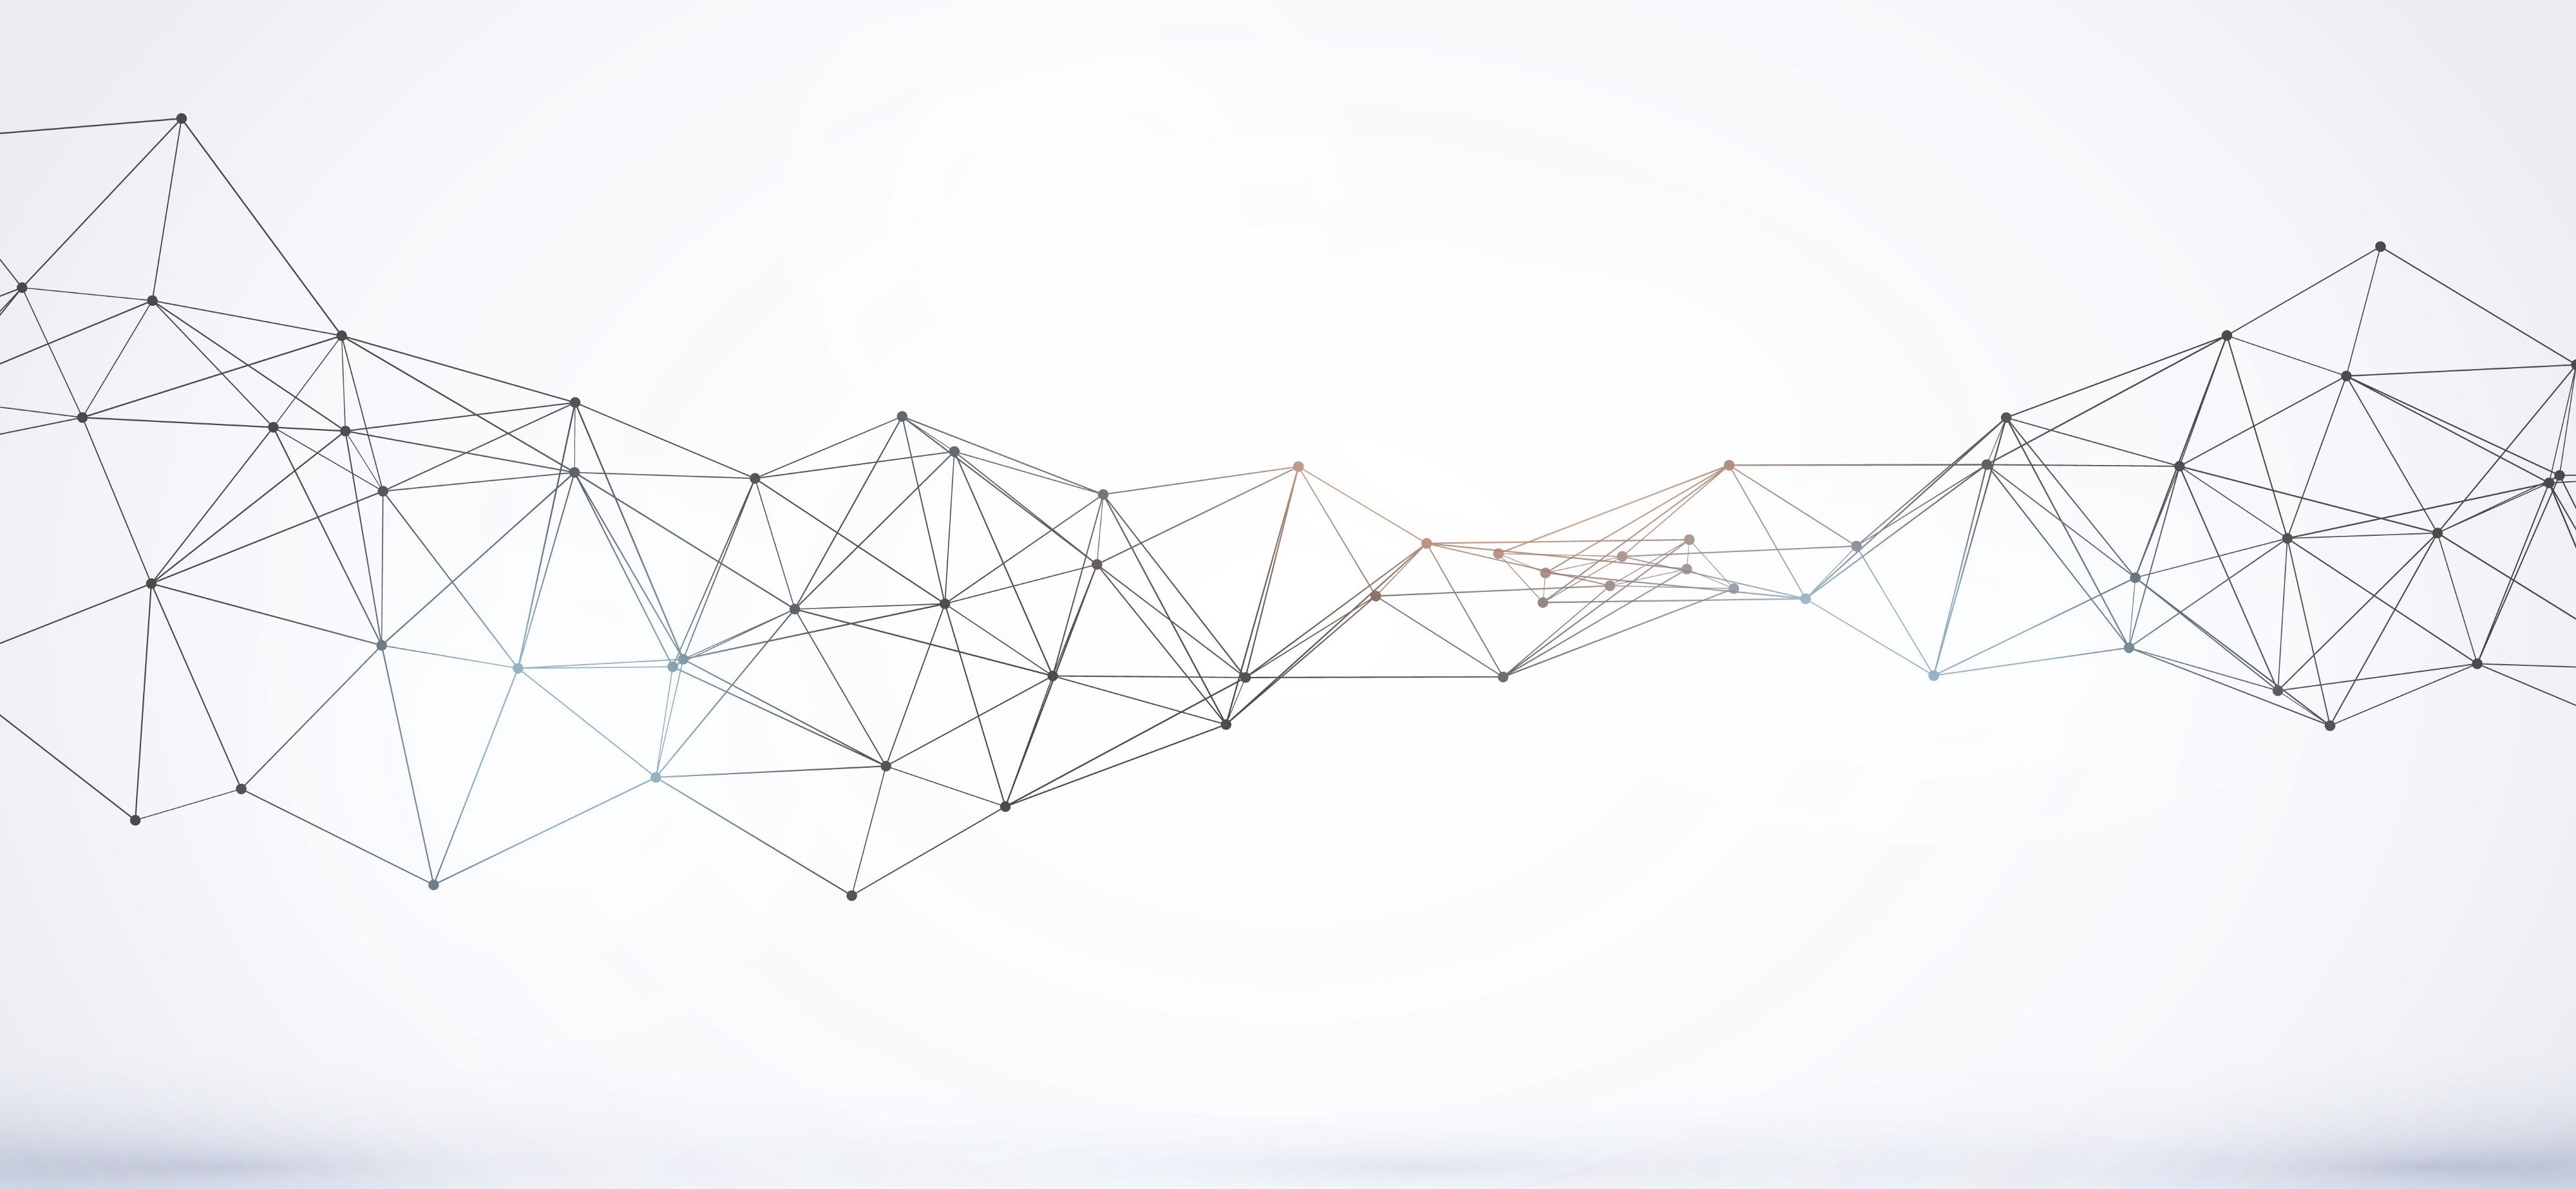
\includegraphics[width=\paperwidth,height=\paperheight]{images/header}};}%
\begin{frame}[plain]
	\vspace{0.5cm}
	\title{\large \begin{spacing}{1.0}Neural Networks for Data Science\end{spacing}\vspace{0.25em}
		\normalsize \begin{spacing}{1.0}\textbf{Master's Degree in Data Science}\end{spacing}\vspace{0.5em}}
	\subtitle{\Large \textbf{Lecture 0: About the course}}
	\date{
		{
\includegraphics[scale=0.8]{images/Uniroma1}}
	}
	\author{
		\setlength{\tabcolsep}{2pt}
		\begin{tabular}{rl}
			\textbf{Lecturer}: & S. Scardapane \\
		\end{tabular}
	}\titlepage
\end{frame}
}

\part{1}

\begin{frame}{Before we start}

	\begin{itemize}
		\item \textbf{Master's Degree in Data Science}, code 10589627, 2nd year, optional group D.
		\item \textbf{Timetable}: Thursdays 09:00--12:00 and Fridays 09:00--11:00, room A5 (Via Ariosto), 24 September -- 18 December 2026. \textbf{Exam dates}: TBD.
		\item \textbf{Office hours}: by appointment, remotely or in person.
	\end{itemize}

	\begin{tcolorbox}
		\href{https://www.sscardapane.it/teaching/nnds-2026/}{https://www.sscardapane.it/teaching/nnds-2026/}
	\end{tcolorbox}

	Register for \textbf{Google Classroom} from the website: it is mandatory for receiving announcements.

\end{frame}

\begin{frame}{Exam ({\color{yellow}new this year})}

	Default exam is an \textbf{oral examination} on the course material (2 questions).

	A \myalert{research project} can replace the oral only when it is agreed in advance and it serves one of two purposes:

	\begin{itemize}
		\item pursuing a mark of \textbf{30 e lode};
		\item preparing for a follow-up \textbf{thesis}.
	\end{itemize}

	It is intended for interested students and is generally \textbf{more demanding} than the oral examination.

\end{frame}

\begin{frame}{The course in one slide}

	\begin{enumerate}
		\item \textbf{Fundamentals}\\
		      Arrays, optimization, supervised learning, MLPs, automatic differentiation, and PyTorch (maybe JAX).
		\item \textbf{Architectures}\\
		      Images, sequences, text, and graphs; convolutions, recurrence, attention, and message passing.
		\item \textbf{Applications}\\
		      Tokenization, pre- and post-training, self-supervised learning, possibly agents.
	\end{enumerate}

\end{frame}

\begin{whiteframe}{Alice in a {\color{yellow}differentiable} wonderland}


	Slides are self-contained, but most of the material is expanded in a textbook:

	\vspace{1em}
	\begin{columns}
		\begin{column}{0.25\textwidth}
			\begin{center}
				{%
					\setlength{\fboxsep}{0pt}%
					\setlength{\fboxrule}{1pt}%
					\fbox{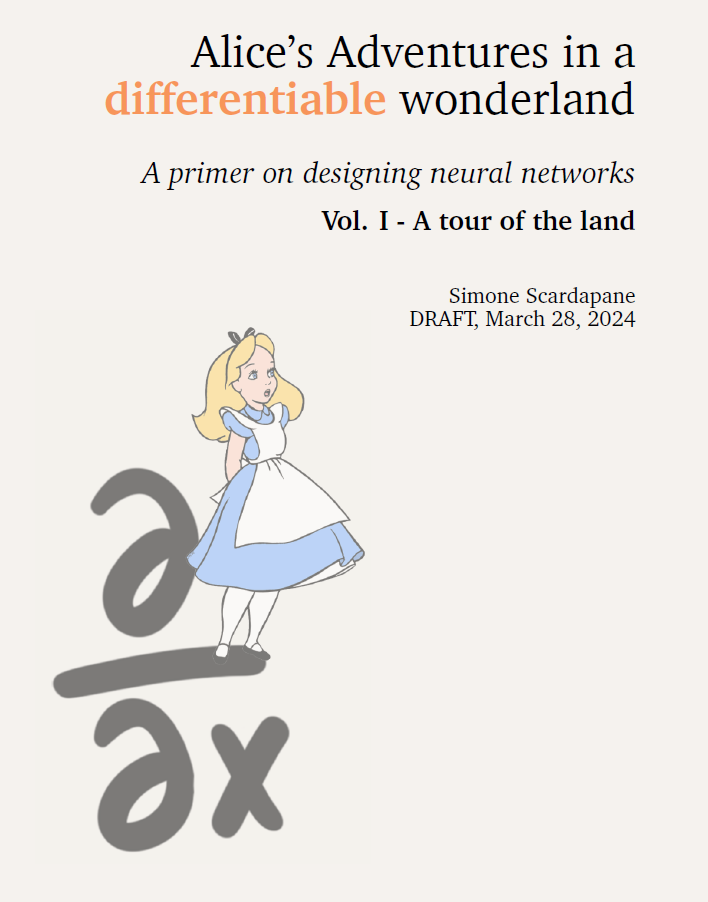
\includegraphics[width=0.2\pagewidth]{images/Alice.png} }%
				}%
			\end{center}
		\end{column}
		\begin{column}{0.75\textwidth}
			The book is available for free as a PDF or as a printed copy:

			\begin{center}\footnotesize\url{https://sscardapane.it/alice-book/}\end{center}

			You can also find additional lab sessions and chapters (e.g., more on post-training of models and automatic differentiation).
		\end{column}
	\end{columns}



\end{whiteframe}

{\setbeamercolor{background canvas}{bg=light-gray}
\begin{frame}{Structured Neural Intelligence Lab}
	\begin{center}
		{\setlength{\fboxsep}{0pt}\setlength{\fboxrule}{1.25pt}%
			\color{darkcerulean}\href{https://www.sscardapane.it/snail/}{\fbox{
\includegraphics[width=0.70\paperwidth]{images/SNAIL_homepage.png}}}}\\[0.4em]
		\small Explore the group: \href{https://www.sscardapane.it/snail/}{www.sscardapane.it/snail}
	\end{center}
\end{frame}
}

\begin{whiteframe}{Optional resource: TinyTorch}
	\begin{columns}[T,onlytextwidth]
		\begin{column}{0.32\textwidth}
			\vspace{0.25em}
			\small
			\textbf{A hands-on implementation of PyTorch from scratch.}

			\vspace{0.5em}
			Explore tensors, layers, and training loops to see what a deep-learning
			library provides.

			\vspace{0.5em}
			\scriptsize\url{https://mlsysbook.ai/tinytorch/}
		\end{column}
		\begin{column}{0.66\textwidth}
			\centering
			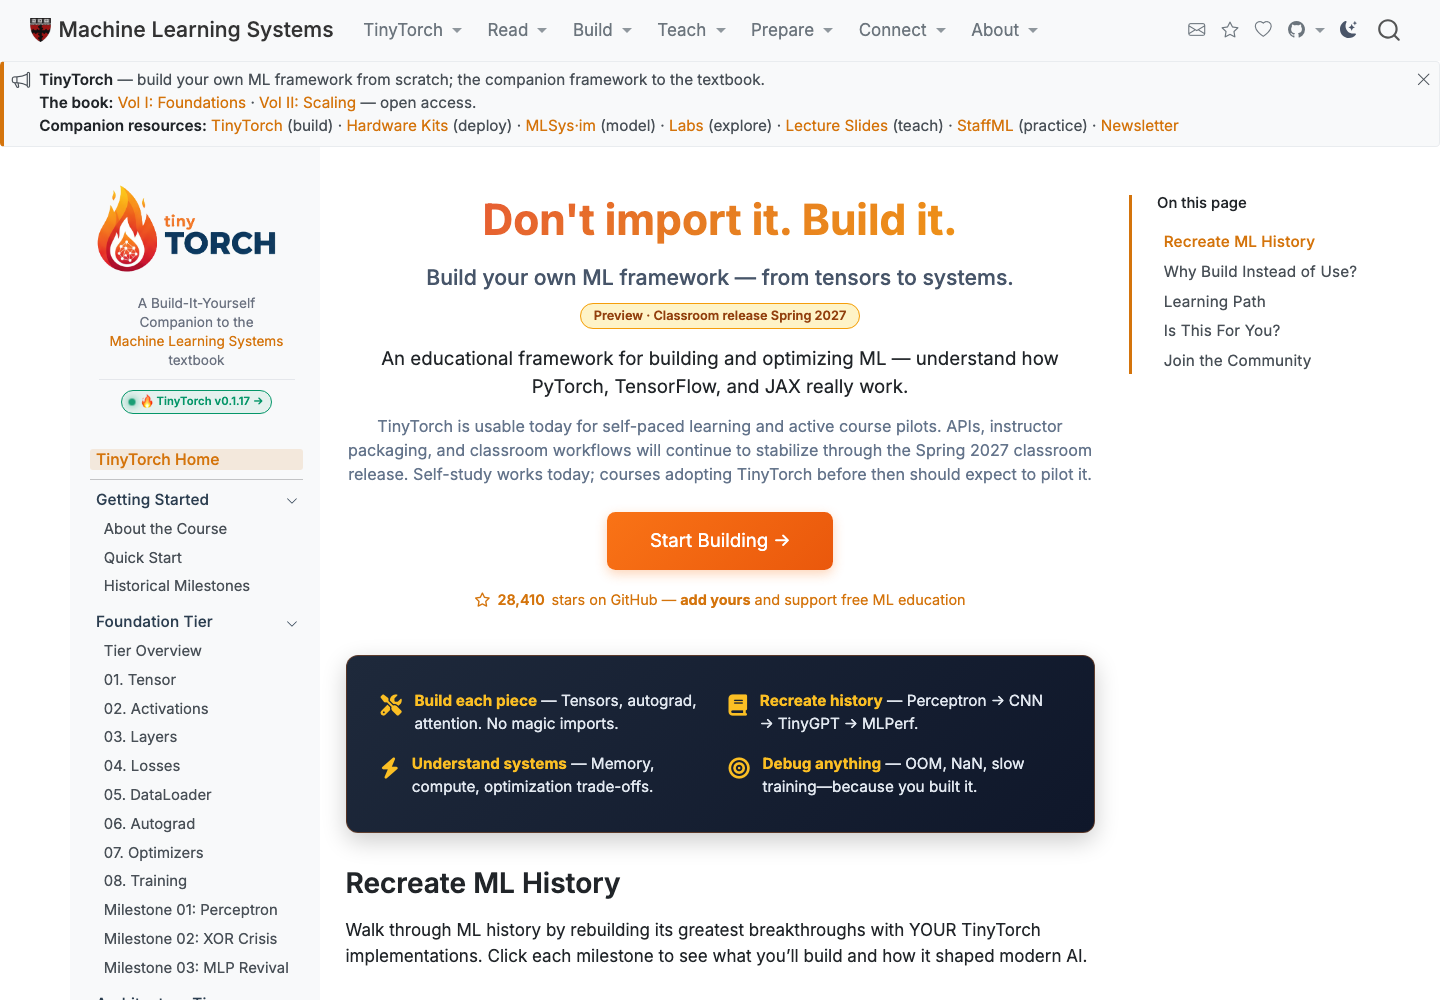
\includegraphics[height=0.48\textheight,keepaspectratio]{images/TinyTorch.png}
		\end{column}
	\end{columns}
\end{whiteframe}

\end{document}
